\subsubsection{エラー率が一定の場合}
まず,$\epsilon$が定数である場合を考える.
このとき,成長条件は$n > n^* = \phi/(k(1-\epsilon))$であることが次のように示せる.

まず,微分方程式で$d/dt=0$として得られる代数方程式から
\begin{align}
  y &= \frac{n}{1+\frac{k+\gamma\phi}{D}x} \\
  c &= \frac{k_1xz}{k_2+\gamma\phi x}
\end{align}
が導かれる.
これを用いて,同様に得られる残り2本の代数方程式から$c$を消去すると,$x\neq 0$なる定常解に対して
\begin{align}
  z &= \frac{\phi(1+\gamma x) - k(1-\epsilon)y}{\frac{k_1k_2}{k_2+\gamma\phi x} - k_1} \\
  z &= \frac{-k\epsilon y}{\frac{k_1k_2}{k_2+\gamma\phi x} - k_1 - \gamma\phi}
\end{align}
がそれぞれ導かれる.
さらに,この二つが等しいとした式から$y$を消去することで,Xの濃度$x$の0以外の定常解は
\begin{equation}
  1-\epsilon \left[1 + \left(\frac{k_2}{k_1 x} + 1 - \frac{\gamma \phi}{k_1}\right)^{-1} \right] = \frac{\phi}{kn}(1+\gamma x)\left(1+\frac{k+\gamma\phi}{D}x\right)
\end{equation}
を満たすと分かる.
さらに$x \ge 0$において,左辺は$x$とともに減少し,右辺は$x$とともに増加することから,定常解$x>0$が存在する条件は,
\begin{equation}
  1-\epsilon > \frac{\phi}{kn}
\end{equation}
と分かる.
したがって,栄養濃度の満たすべき条件は
\begin{equation}
  n > n^* = \frac{\phi}{k(1-\epsilon)} \label{nast_errconst}
\end{equation}
と求まる.

この式は,代謝物Xの消費反応の速度定数が$\phi$,生成反応の実効的な速度定数が$k(1-\epsilon)$となることから説明できる.
また,反応$\ce{Z + X <=> C}$はここでは効いていないことが分かる.

しかし,この証明のような解析的な手法では,式\eqref{nast_errconst}が成り立つときに$x>0$を満たす定常解が安定であること(成長速度が正の値で安定すること)を示すのが難しかった.
そこで次に,数値計算によって式\eqref{nast_errconst}と成長速度が正であることが等価であることを部分的に確認した.
ここでは,パラメータ$k,k_1,k_2,\phi,\gamma,D$はすべて1とした.
まず,外部栄養濃度$n$をある値に固定し,$\epsilon=0,0.2,0.4,0.6,0.8$のそれぞれについて,初期濃度を$x=y=1, z=c=0$として十分な時間(時刻$t=10^5$まで)シミュレーションを行った.
その結果,最終的にすべての成分濃度と成長速度$\mu$が定常となっていることを確認した.
このとき,外部栄養濃度$n$と定常成長速度$\mu$の関係は図\ref{fig:n_vs_mu_errconst}のようになった.
この図を参考に,定常成長速度が$\mu > 10^{-3}$となる最小の外部栄養濃度$n^*$を「成長に必要な栄養濃度」と考えることにした.
そこで,外部栄養濃度$n$を0から0.1ずつ増加させ,$\mu>10^{-3}$となる最小の$n$を$n^*$として,$\epsilon$と$n^*$の関係をプロットした(図\ref{fig:err_vs_n_errconst}).
この図から,理論式\eqref{nast_errconst}はこの数値計算の結果と整合することが確認できる.

\begin{figure}[htbp]
  \centering
  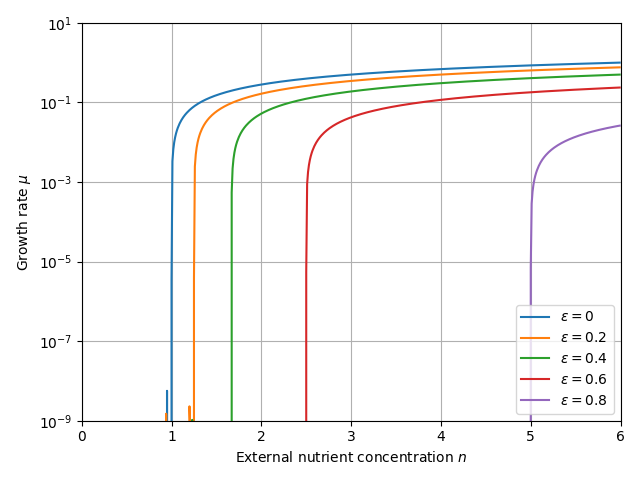
\includegraphics[width=10cm]{n_vs_mu_errconst.png}
  \caption{エラー率を定数($\epsilon=0,0.2,0.4,0.6,0.8$)として計算した,時刻$t=10^5$における外部栄養濃度$n$と成長速度$\mu$の関係(初期濃度は$x=y=1, z=c=0$,時間の刻み幅は0.1,$n$の刻み幅は0.01,その他のパラメータ$k,k_1,k_2,\phi,\gamma,D$はすべて1とした.).この結果は式\eqref{nast_errconst}と整合する.}
  \label{fig:n_vs_mu_errconst}
\end{figure}

\begin{figure}[htbp]
  \centering
  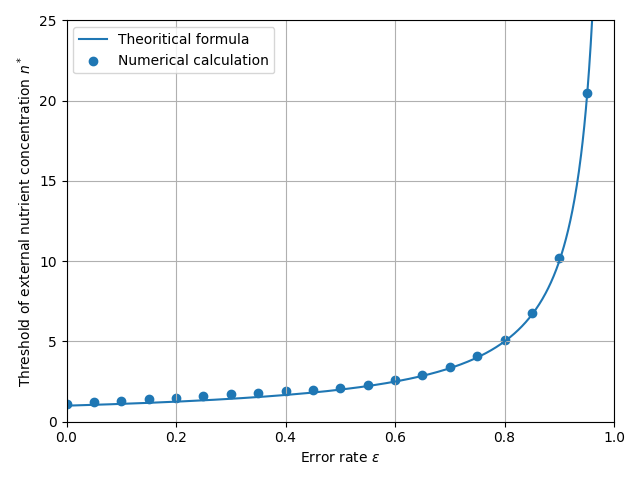
\includegraphics[width=10cm]{err_vs_n_errconst.png}
  \caption{エラー率が定数であるとして計算した,$\epsilon$と成長に必要な($\mu > 10^{-3}$となる最小の)外部栄養濃度$n^*$の関係(Numerical calculationとして示したプロット.$n^*$を求めるにあたって,$n$は刻み幅0.1で変更した.それ以外のパラメータは図\ref{fig:n_vs_mu_errconst}と同様である.).これは式\eqref{nast_errconst}で表される理論線(Theoritical formulaとして示した曲線)と整合している.}
  \label{fig:err_vs_n_errconst}
\end{figure}